%-----------------------------------------------------------
% From [this answer](https://tex.stackexchange.com/a/708673/64441).
%-----------------------------------------------------------

\documentclass{article}

\usepackage{tikz}
\usepackage{animate}

\newlength{\step}
\setlength{\step}{\dimexpr 10cm / 18 \relax}

\newcommand\playgo[3]{\ifnum#1<#2\phantom{#3}\else#3\fi}

\begin{document}
  \begin{animateinline}[step,controls=step]{1}
    \multiframe{4}{i=0+1}{
      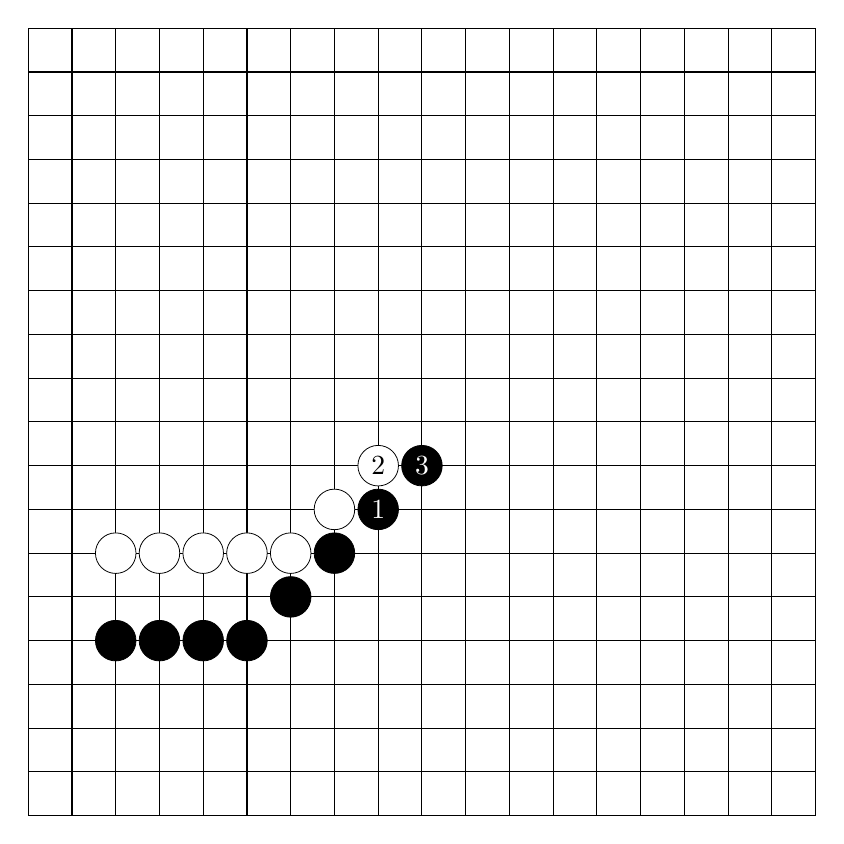
\begin{tikzpicture}[x=\step,y=\step]
        %create the board 
        \draw[step=1] (0, 0) grid (18, 18);

        %setup black
        \foreach \bloc in {{2,4},{3,4},{4,4},{5,4},{6,5},{7,6}}{
          \filldraw[line width = 0.1mm] (\bloc) circle [radius = 0.2575cm];
        }

        %setup white
        \foreach \wloc in {{2,6},{3,6},{4,6},{5,6},{6,6},{7,7}}{
          \filldraw[fill=white,line width = 0.1mm] (\wloc) circle [radius = 0.2575cm];
        }

        %play the go-game start from black
        \foreach \stepnum/\loc in {1/{8,7},2/{8,8},3/{9,8}}{
          \playgo{\i}{\stepnum}{\filldraw[fill={\ifodd\stepnum black\else white\fi},line width = 0.1mm] (\loc) circle [radius = 0.2575cm] node [color = \ifodd\stepnum white\else black\fi] {\stepnum};}
        }
      \end{tikzpicture}
    }
  \end{animateinline}
\end{document}

